\chapter{\IfLanguageName{dutch}{Resultaten}{Results}}%
\label{ch:resultaten}

In dit hoofdstuk worden de resultaten uit de requirementsanalyse, vergelijkende studie en de ontwikkeling van het prototype besproken. 

\section{Requirementsanalyse}

Woorden- en synoniemenlijsten kunnen een ondersteunend middel aanbieden voor zowel scholieren met dyslexie als zonder bij het lezen van wetenschappelijke artikelen en wordt aangeboden in Kurzweil. Automatisch genereren is enkel prevalent bij ChatGPT en de Bing chatbot, maar de tools houden geen rekening met de doelgroep, tenzij expliciet aangegeven met een \textit{one-shot summary}. Andere tools houden helemaal geen rekening met de doelgroep en kunnen enkel woordenlijsten genereren op basis van gekozen woorden.

\medspace

In figuur \ref{img:tryout-bing-ai} wordt er een online wetenschappelijk artikel meegegeven. Er wordt geen titel of onderwerp meegegeven, maar de Bing AI chatbot is in staat om een abstraherende samenvatting te maken van het artikel. Daarna kan de chatbot meer uitleg geven over een bepaald onderwerp, alsook de referenties naar de oorspronkelijke bron meegeven. 

\begin{figure}[H]
	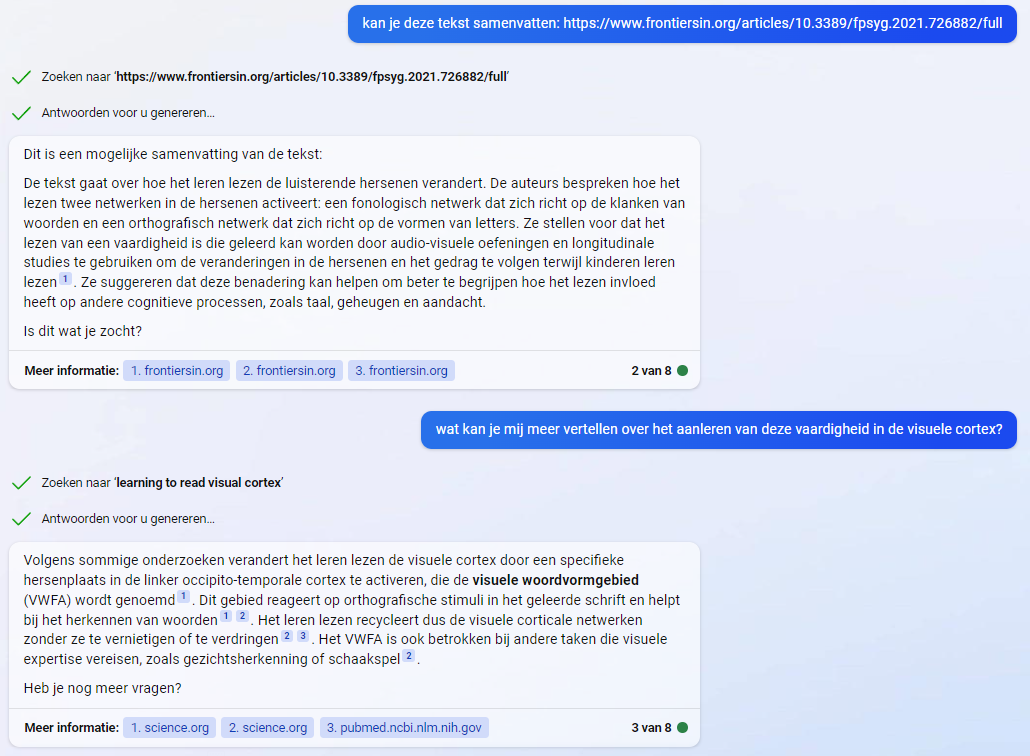
\includegraphics{img/bing-ai-chatbot-example.png}
	\caption{Resultaat Bing Chatbot}
	\label{img:tryout-bing-ai}
\end{figure}

\medspace

Met de huidige erkende softwaretools in het onderwijs is het moeilijk om syntactische vereenvoudiging toe te passen op wetenschappelijke artikelen. Online webtoepassingen bieden weliswaar mogelijkheden om de moeilijkheidsgraad van de zinsstructuur te verlagen, maar ze zijn voornamelijk gericht op het verkorten van de oorspronkelijke tekst, of het maken van een samenvatting. Het aanpassen van tangconstructies, verwijswoorden, voorzetseluitdrukkingen, samengestelde werkwoorden en onregelmatige werkwoorden blijft daarom een uitdaging voor deze toepassingen. Zelfs het schrijven in de actieve stem kan problematisch zijn, en de beschikbare prompts zijn beperkt tot vooraf gedefinieerde transformaties.

\medspace

Het uploaden van een PDF wordt beschouwd als een onmisbare optie bij de geteste tools, maar ChatGPT en Bing Chat beschikken niet over deze functie. De software die wordt gebruikt in het onderwijs kan geen tekst uit PDF's extraheren, in tegenstelling tot webtoepassingen die deze mogelijkheid wel bieden. De geteste tools zijn voornamelijk gericht op samenvatting van teksten. Hoewel ChatGPT en Bing Chatbot teksten kunnen genereren in een schrijfstijl vergelijkbaar met die van mensen, zijn ze niet in staat om PDF's te verwerken. Het kopiëren en plakken van tekst uit het originele document kan leiden tot fouten en is omslachtig, daarom moet er worden gewerkt aan verbetering van deze werkwijze. Bestaande tools hebben moeite met het extraheren van tekst uit oudere PDF's, dus het prototype moet een oplossing bieden voor dit mogelijke probleem.

\medspace

Uitgezonderd van Simplish en Rewordify bieden de uitgeteste tools geen ingebouwde tekstanalysemodule en bieden onvoldoende inzicht op leesgraadsmetrieken van zowel het ingegeven document als het vereenvoudigde document. Simplish steekt boven de rest uit door aan de hand van kleurcodes criteria over de vereenvoudigde tekst mee te geven, waaronder niet-veranderende woorden, adequate vertalingen, uitleg naar de voetnoot, homoniemen of woorden die geen eenvoudigere synoniemen hebben. Zoals aangegeven in \ref{img:simplish-output} duidt de vergelijkende weergave de verschillen aan tussen de oorspronkelijke en vereenvoudigde tekst en met behulp van kleurcodes worden de verschillende transformaties aangegeven. Scholarcy vult hierop aan en biedt meer inzichten in de leesbaarheidsgraad van de vereenvoudigde tekst, zoals geïllustreerd in \ref{img:scholarcy}.

\begin{figure}[H]
	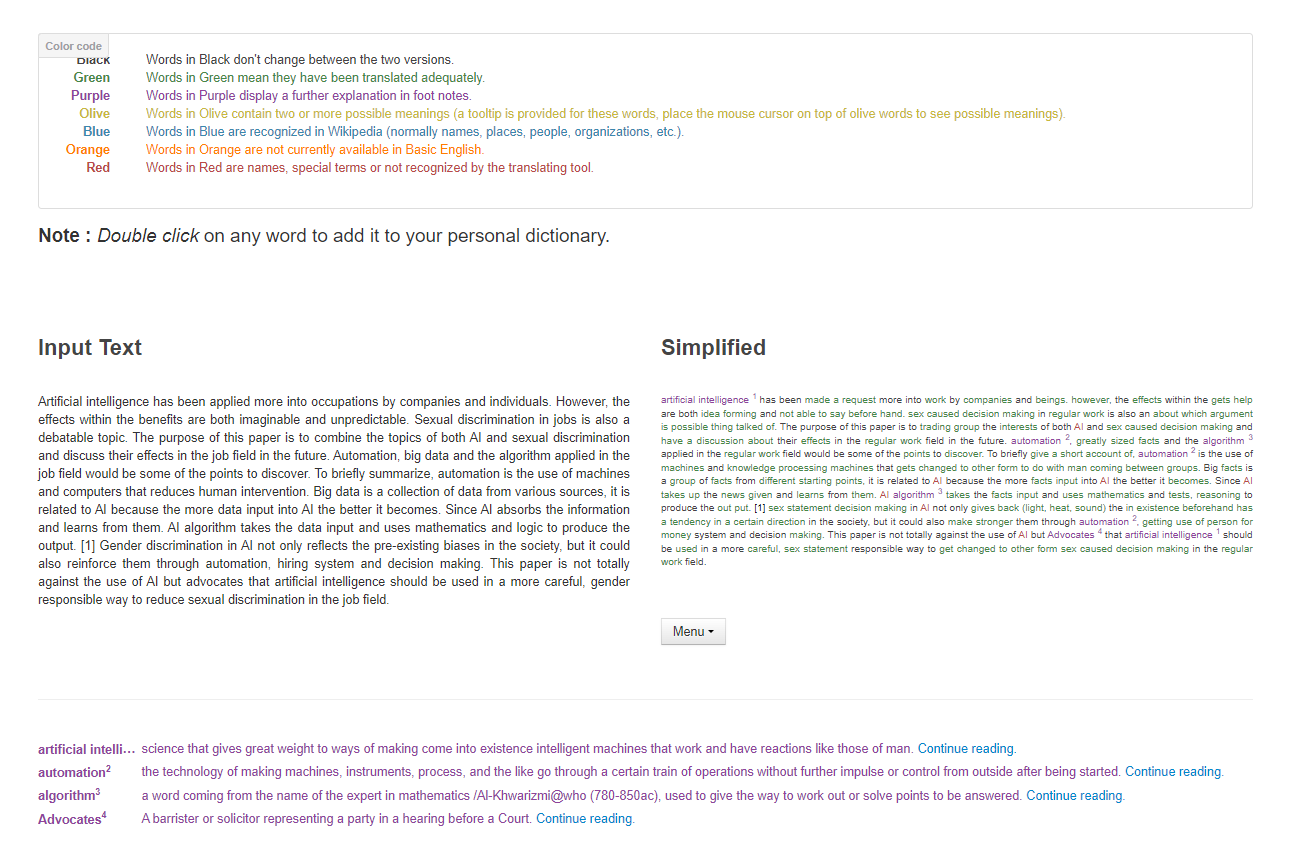
\includegraphics[width=\linewidth]{img/simplish-output.png}
	\caption{Illustratie van de tekstanalyse bij Simplish na een tekstvereenvoudiging.}
	\label{img:simplish-output}
\end{figure}

\begin{figure}[H]
	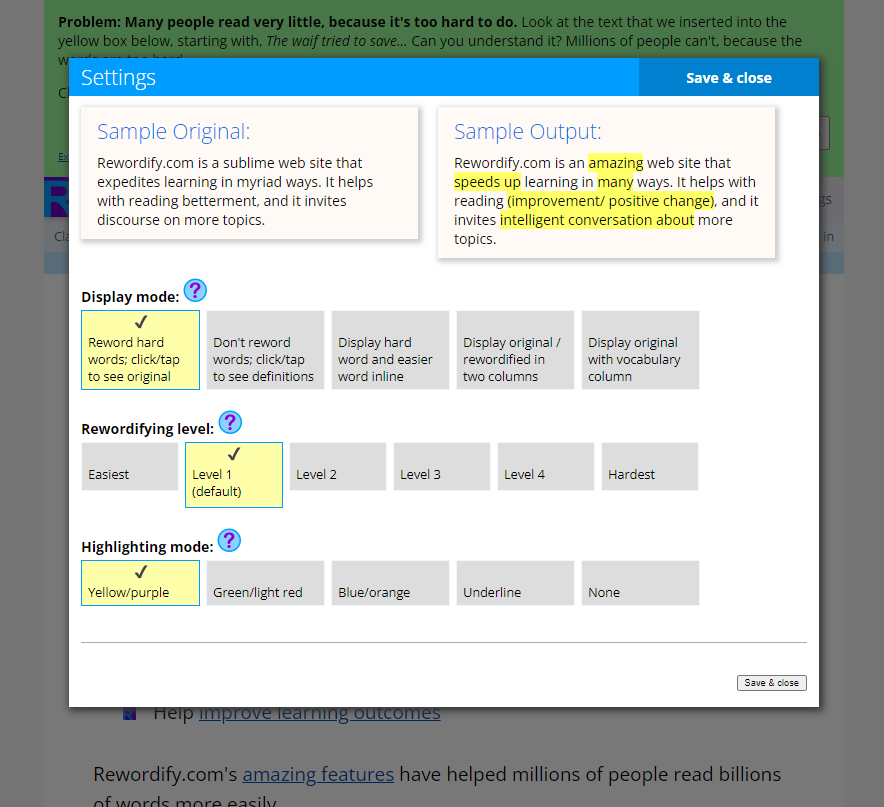
\includegraphics[width=\linewidth]{img/scholarcy-attempt.png}
	\caption{Illustratie van de tekstanalyse bij Rewordify.}
	\label{img:scholarcy}
\end{figure}

De requirementsanalyse neemt geen functionaliteiten op van obscure proof-of-concepten. Deze ontbreken de nodige testen en zekerheid dat deze effectieve gepersonaliseerde en geautomatiseerde tekstvereenvoudiging aanbieden. Twee van de online tools, namelijk Resoomer en Scispace, bieden uitsluitend samenvattingsfunctionaliteiten aan. Resoomer is sneller geneigd om de belangrijkste zinnen te markeren en vervolgens deze in een kortere tekst terug te geven. Dit kan een effect hebben op de betrouwbaarheid van de functionaliteiten, alsook op de leesgraadmetrieken.

\begin{figure}[H]
	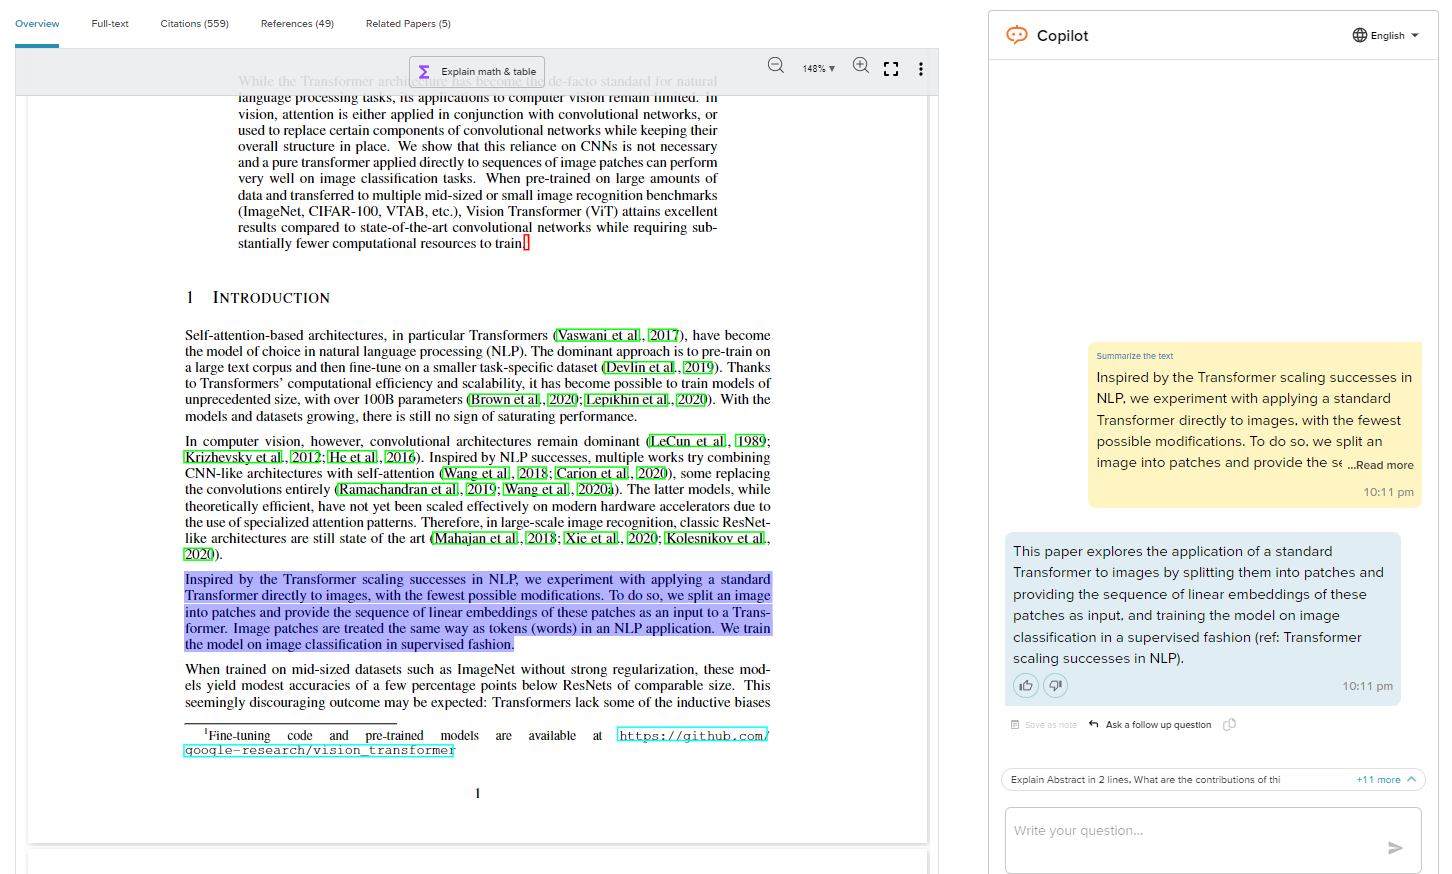
\includegraphics{img/typeset-example.png}
	\caption{Schermafbeelding van SciSpace}
	\label{img:scispace-example}
\end{figure}

\section{Vergelijkende studie}

Modellen T1, T2 en T3 zijn, zoals verwezen in de bijlage, niet in staat om syntactische vereenvoudiging op een tekst toe te passen. Enkel T4 kan via prompt P2, P3, P4, P5 en P6 de syntax van een zin verlagen. Alle uitgeteste taalmodellen zijn echter wel in staat om lexicale vereenvoudiging te realiseren, al wordt de inschatting van de doelgroep in twijfel getrokken. De referentieteksten schatten de doelgroep correct in, door reeds gekend jargon niet aan te passen, maar nieuwe jargon wel aan te passen naargelang er een beschikbaar synoniem is.

\medspace

De modellen T1, T2 en T3 zijn niet in staat om syntactische vereenvoudiging op een tekst toe te passen. Alleen T4 kan via de prompts P2, P3, P4, P5 en P6 de zinsstructuur verlagen. Hoewel alle geteste taalmodellen in staat zijn om lexicale vereenvoudiging te realiseren, wordt de nauwkeurigheid van de doelgroepsinschatting in twijfel getrokken. De referentieteksten schatten de doelgroep correct in door bekend jargon niet aan te passen, maar wel nieuwe jargon aan te passen als er een beschikbaar synoniem is. 

\medspace

In tegenstelling tot GPT-3 zijn de modellen T1, T2 en T3 niet in staat om het formaat van de uitvoer aan te passen. De uitvoer blijft een doorlopende tekst. In de referetietekst past één van de auteurs het formaat aan naar tabelvorm voor enkele paragrafen, waar de inhoud beter in tabelvorm kan gestructureerd worden. Alleen bij de prompts P5 en P6 wordt er expliciet gevraagd om een formaatwijziging, anders geeft T4 vrijwel altijd een doorlopende tekst terug. Zonder de expliciete aanduiding is het model niet in staat om dit zelf te bepalen. Verder onderzoek moet uitwijzen of T4 in staat is om zelfstandig deze bepaling kan maken, zo niet kan deze formaatwijziging niet automatisch bepaald worden en is er tussenkomst van de eindgebruiker vereist. Dit moet ook zo opgenomen worden als een functionaliteit in het prototype.

\medspace

Tijd speelt ook een rol en zowel aangesproken per API, als lokaal draaiend, scoren T1 en T2 ondermaats. Dit kan oplopen tot hoogstens 30 seconden voor een zin van tien tot dertig woorden, vergeleken met T3 die dezelfde zin in minder dan 10 seconden kan vereenvoudigen.

\medspace

Hoewel T3 in staat is om zinsyntaxtransformaties uit te voeren, ervaart deze problemen ondervinden bij het verwerken van alle meegegeven transformaties. Het taalmodel kan transformaties ontbreken als alle transformaties in één prompt zijn betrokken. Een voorgestelde aanpak om dit tegen te gaan, bestaat uit een pipeline van hoogstens drie prompts die elkaar opvolgen, zoals geïllustreerd in figuur ...

\medspace

Ontwikkelaars hebben toegang tot T1, T2 en T3 via HuggingFace voor lexicale vereenvoudigingstaken. Deze taalmodellen zijn echter ontoereikend voor gepersonaliseerde tekstvereenvoudiging en daarom is T4 een geschikter model voor het vereenvoudigen van wetenschappelijke artikelen op maat. GPT-3 presteert goed op gepersonaliseerde vereenvoudigingstaken, maar het is belangrijk om op te merken dat geen enkel taalmodel de doelgroep altijd nauwkeurig kan inschatten. Extra trainingsdata, zoals leerstof of wetenschappelijke artikelen die wel op het niveau van een 16-18-jarige is geschreven, kan het model steunen bij de doelgroepsinschatting. Het gebruik van Engelstalige prompts waarin expliciet de gewenste uitvoertaal wordt vermeld, resulteert in coherentere teksten dan bij een Nederlandstalige prompt.

\section{Opbouw van het prototype}

Het prototype voldoet aan alle functionaliteiten die zijn gespecificeerd in het Moscow-schema \ref{img:moscow}. Het overtreft daarmee elke andere tool uit de requirementsanalyse op alle gebieden. Het is vooral op het gebied van formaatwijzigingen de beste, wat suggereert dat het prototype de huidige staat van deze toepassingen weergeeft, gezien de consistente ontwikkeling van de personalisatieopties. Op het gebied van tekstvereenvoudiging scoort het prototype vergelijkbaar of iets beter dan wat GPT-3 kan, wat voor zich spreekt aangezien het twee identieke taalmodellen zijn.

\medspace

Ontwikkelaars kunnen de opgebouwde flowchart volgen om team van vier rollen, namelijk systeem, data, NLP en web ontwikkelaars, te begeleiden doorheen de ontwikkeling van een toepassing voor tekstvereenvoudiging. De flowchart benadrukt dat deze handelingen ook perfect parallel kunnen worden uitgevoerd. Jupyter notebooks bieden een ontwikkelaarsvriendelijke manier om de code vooraf met eenduidige visuele feedback te kunnen testen.

\medspace

Dit prototype maakt geen gebruik van lokaal gehoste taalmodellen. Zo vermindert de nodige rekenkracht en geheugenruimte op het systeem waarop het prototype draait in vergelijking met een lokaal gehost taalmodel. Wanneer ontwikkelaars de toepassing willen uitrollen naar het grote publiek, kunnen ze overschakelen naar lokaal gehoste taalmodellen in plaats van taalmodellen per API. Door de taalmodellen verder te finetunen en te trainen op meer datasets, kunnen AI-ontwikkelaars betere resultaten behalen. 

\medspace

Het ontwikkelen van gebruikersvriendelijke handelingen kan gemakkelijk en snel worden ontwikkeld met behulp van HTML, CSS en JavaScript, zonder de nood van een complex framework. Uit onderzoek blijkt echter dat deze methoden eenvoudig te ontwikkelen zijn, zelfs door pas afgestudeerde bachelorstudenten. AI-softwarebedrijven zouden meer moeten inzetten op personalisatie-opties voor scholieren met dyslexie in de derde graad van het middelbaar onderwijs, omdat zij momenteel het meest betrokken zijn bij de digitalisering. Later kunnen softwareontwikkelaars overgaan op een complexer of robuuster framework. Verder onderzoek is nodig naar het ideale framework om een gepersonaliseerde weergave mogelijk te maken, aangezien dit momenteel nog wordt gedaan met handmatige JavaScript-functies. Een front-end framework dat dit alles beheert, zou handiger zijn voor webontwikkelaars.

\medspace

Dit prototype is momenteel alleen beschikbaar in een lokale omgeving en kan nog niet worden gebruikt door het grote publiek. Het prototype kan teksten lexicaal en syntactisch vereenvoudigen wanneer deze in PDF- of volledige tekstformaat worden ingevoerd. Het prototype heeft functionaliteit voor zowel docenten als studenten, die elk verschillende prioriteiten hebben. Hoewel testen nog nodig zijn, wordt dit wel aangeraden. Onderzoekers op het gebied van logopedie kunnen het prototype testen bij studenten met dyslexie na een (begeleide) installatie van de vereiste set-up. Ook onderzoekers op het gebied van onderwijs kunnen dit gebruiken om de meningen van zowel studenten als docenten te verzamelen en zo de effectiviteit van het prototype te beoordelen. Deze experimenten zijn belangrijk omdat ze kunnen wijzen op de effectiviteit van het prototype.

